\documentclass[colorthm]{./civarticle}
\usepackage{graphicx} % Required for inserting images
\usepackage[math]{blindtext}
\usepackage{float}

\title{esse}
\author{Назаров Захар}
\date{December 2023}

\begin{document}


\section{Введение}

В данной работе дается описание и некоторые аспекты безопасности следующих поточных шифров: RC4, Snow3G, SEAL, MUGI, семейство шифров A5(A5/1, A5/2 и A5/3) И LILI128. Устройство шифра LILI128 и его особенности рассматриваются более детально, также описаны 3 атаки на него.

\section{Термины и определения}

Для понимания работы требуется ознакомиться со следующими определениями:

\begin{definition}
  Булева функция называется сбалансированной, если количество наборов переменных, на которых она принимает значение 0, равно количеству наборов переменных, на которых она принимает значение 1.
\end{definition}

\begin{definition}
  Нелинейностью (nonlinearity) булевой функции f степени n является значение минимального расстояния по Хеммингу до линейной функции:
  \begin{equation}
      N_f=\min _{g \in \mathcal{A}_n} d_H(f, g)
  \end{equation}
  , где $\mathcal{A}_n$ - пространство линейных функции степени n, $d_H$ - расстояние по Хеммингу между столбцами со значениями булевых функции.
\end{definition}

\begin{definition}
  Регистр сдвига, или сдвиговый регистр (англ. shift register) представляет собой устройство, состоящее из последовательно соединенных триггеров (по сути ячеек, хранящих 0 или 1)
\end{definition}

Основной функцией регистра сдвига является последовательное сдвигание разрядов (битов)  внутри него, после которого обычно снимается выходной бит для дальнейшего использования. Это сдвигание происходит в ответ на тактовый сигнал.

\begin{definition}
  Регистр сдвига с линейной обратной связью (РСЛОС, англ. linear feedback shift register, LFSR) — сдвиговый регистр, у которого значение входного бита равно линейной булевой функции от значений всех битов регистра до сдвига.
\end{definition}

\begin{figure}[H]
    \centering
    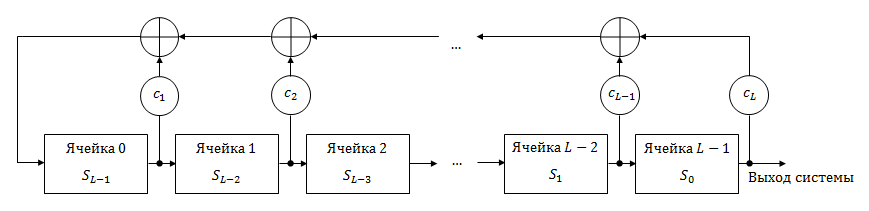
\includegraphics[width=0.75\linewidth]{LFSR3.png}
    \caption{Регистр сдвига с линейной обратной связью}
    \label{fig:enter-label}
\end{figure}

\begin{definition}
  Определим линейную сложность L(s) бинарной бесконечной последовательности s:
  \begin{enumerate}
        \item Если s - это последовательность из нулей, то L(s) = 0.
        \item Если не существует LFSR, генерирующего s, то L(s) = $inf$
        \item Если существует хотя бы один LFSR, генерирующий s, то L(s) - это длина самого короткого LFSR, который генерирует s.
    \end{enumerate}
\end{definition}

\begin{figure}[H]
    \centering
    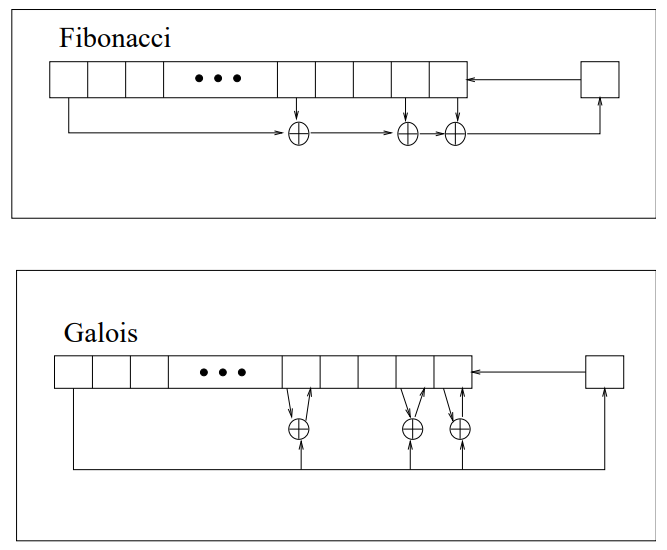
\includegraphics[width=0.75\linewidth]{фибо_галуа.png}
    \caption{Конфигурация Фибоначчи и конфигурация Галуа}
    \label{fig:enter-label}
\end{figure}

\begin{definition}
  Конфигурация Фиббоначи - это способ реализации LSFR, при котором есть одна функция обратной связи. За 1 такт работы регистра происходит вычисление первого бита с помощью этой функции, а также сдвиг регистра.
\end{definition}

\begin{definition}
  Конфигурация Галуа - это способ реализации LSFR, при котором для каждой ячейки есть своя функция обратной связи. За 1 такт работы регистра происходит обновление каждой ячейки с помощью своей функции, а также сдвиг регистра.
\end{definition}

\begin{remark}
    Так как глубина схем обратной связи для отдельных битов обычно меньше, чем для функции обратной связи 
    в конифгурации Фибоначчи, то для конфигурации Галуа время 1 такта может быть уменьшено [2].
\end{remark}

\begin{definition}
  Корреляционная атака (или атака типа "разделяй и властвуй") - это класс атак на основе открытых текстов для взлома потоковых шифров, ключевая последовательность которых генерируется путем объединения вывода нескольких LSFR (но не всех) с использованием логической функции.
\end{definition}

\begin{definition}
  Быстрая корреляционная атака [4] (англ. fast correlation attack, fca) - это корреляционная атака, которая происходит существенно быстрее чем обычная корреляционная атака за счет того, что проблему рассматривают в контексте теории кодирования.
\end{definition}

\begin{definition}
  Атака компромисса между временем/памятью/данными (time-memory tradeoff atack) на потоковые шифры [7] - тип криптографической атаки, в которой заранее вычисляется таблица, содержащая пары вида (начальное состяние, ключевая последовательность фиксированной длины для этого состояния), и затем производится поиск подпоследовательности ключевой последовательности в этой таблице. При попадании в таблицу с высокой вероятностью, соотвествующее начальное состояние является правильным. Такое название объясняется тем, что злоумышленник ищет компромисс между памятью, которая у него есть, наблюдаемыми данными и количеством операции, ведь улучшение одного параметра ведет к ухудшению другого.
\end{definition}

\begin{definition}
  Сеть Фейстеля - это одна из архитектур блочного шифра. Исходный текст делится на блоки, и над каждым блоком производится одно и тоже преобразование. На вход этому преобразованию подается блок и ключ. Вот так выглядит это преобразование: 

  \begin{figure}[H]
      \centering
      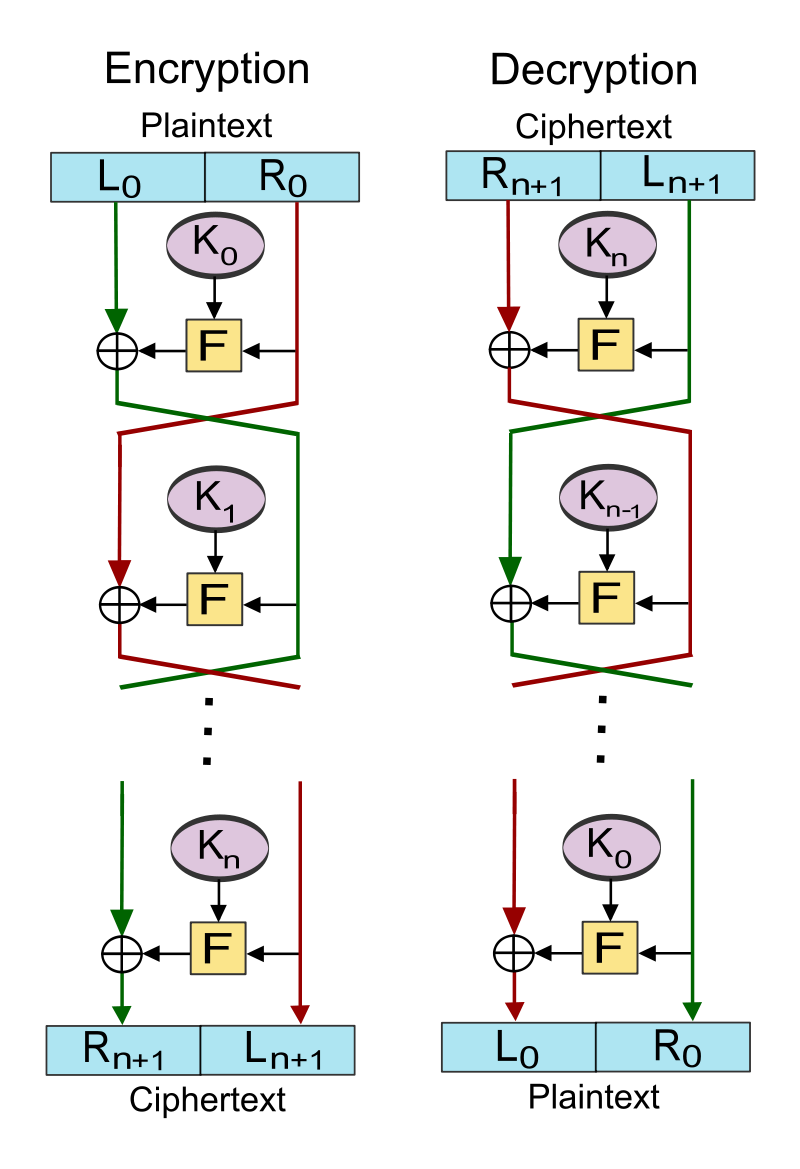
\includegraphics[width=0.5\linewidth]{800px-Feistel_cipher_diagram_en.svg.png}
      \caption{Сеть Фейстеля [17]}
      \label{fig:enter-label}
  \end{figure}

    Исходный текст (блок) делится на две части: $R_0, L_0$. Из ключ создаются подключи, количество которых ровно количеству раундов. Один раунд выглядит следующим образом:
    \begin{enumerate}
        \item $L_i = R_i \oplus F(L_{i-1}, K_{i-1})$
        \item $R_i = L_i$
    \end{enumerate}

    Происходит N раундов, и $(L_n, R_N)$ является выходом преобразования. Функция $F$ может быть разной. Расшифрование происходит в обратном порядке.
  
\end{definition}

\begin{definition}
    Пусть у нас есть семейство функции $F(k, x)$, где $k$ - это параметр, а $x$ - переменная. Для каждого $k$ определена функция $F_k(x)$, которые действуют из множества A в множество B. Функция $F(k, x)$, при случайном и равновероятном выбранном $k$ называется псевдослучайной, если $F_k(x)$ неотличима (за разумное время) от истинно случайной функции, действующей из A в B.
\end{definition}

\section{RC4}
В 1987 году сотрудник компании RSA Security Рональд Ривест создал потоковый шифр RC4. В течение 7 лет шифр являлся коммерческой тайной. Вскоре описание RC4 было опубликовано в группе новостей usenet.

\subsubsection{Описание шифра RC4}

RC4 генерирует ключевую последовательность длины сообщения, которая затем накладывается на исходное сообщение и получается шифротекст. На вход алгоритму подаются 2 параметра: секретный ключ $K$ длиной $l$ байт (которая не может быть больше 256 байт) и $n$ - длина выходной ключевой последовательности. Затем идут 2 этапа: инициализация и генерация ключевой последовательности.

\textbf{Инициализация генератора}

С помощью секретного ключа $K$, генерируется случайная подстановка длины $n$ следующим образом:

\begin{figure}[H]
    \centering
    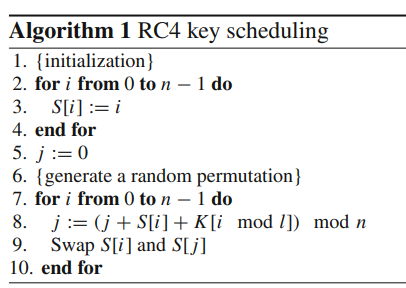
\includegraphics[width=0.5\linewidth]{Снимок экрана 2024-01-12 162647.png}
    \caption{Инициализация RC4 [29]}
    \label{fig:enter-label}
\end{figure}

\textbf{Этап генерации ключевой последовательности}

Генерация ключевой последовательности происходит следующим образом:

\begin{figure}[H]
    \centering
    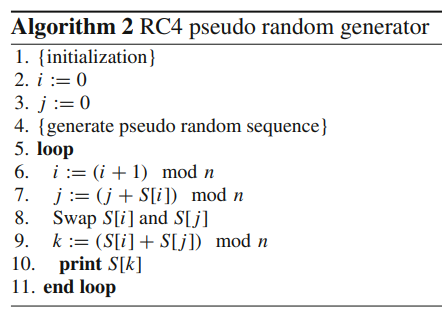
\includegraphics[width=0.5\linewidth]{Снимок экрана 2024-01-12 163228.png}
    \caption{Генератор псевдослучайной последовательности RC4 [29]}
    \label{fig:enter-label}
\end{figure}

\subsubsection{Безопасность шифра}
В 2007 году было показано [30], что первый байт ключевого потока коррелирован с первыми тремя байтами ключа. В 2015 году была представлена реальная атака на протокол TLS, испольщующий RC4 [31]. C помощью около $2^{27}-2^{30}$ пар открытого текста и шифротекста за 52 часа они смогли восстановить ключ.

\section{Snow3G}

Шифры семейства Snow были разработаны Лундским Университетом (Швеция) для безопасной передачи мобильных данных. В 2006 году была выпущена новая версия шифра Snow - Snow3G [27]. Это поточный шифр, работающий в синхронном режиме, который производит ключевую последовательность, кратную 32-битам.

\subsubsection{Описание шифра Snow3G}

Потоквый шифр Snow3G принимает на вход 2 параметра: 128-битный секретный ключ и 128-битный инициализирующий вектор. Шифр имеет 608-битное внутреннее состояние, которое формируются двумя компонентами: регистром и конечным автоматом (finite state machine, FSM). Схема Snow3G выглядит следующим образом:

\begin{figure}[H]
    \centering
    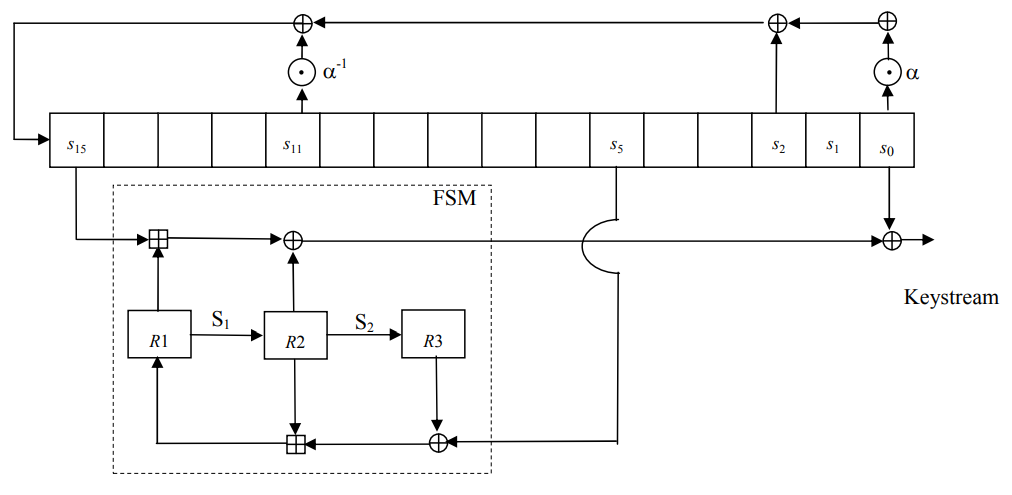
\includegraphics[width=1\linewidth]{Снимок экрана 2024-01-12 141248.png}
    \caption{Enter Caption}
    \label{fig:enter-label}
\end{figure}

Регистр является LSFR и состоит из 16 32-битных ячеек. Функция обратной связи выглядит так: 

\begin{equation}
    s_{t+16} = \alpha * s_t \oplus s_{t+2} \oplus \alpha^{-1}*s_{t+11}. \alpha \in [0, \dots, 2^{32}-1]
\end{equation}

\textbf{Тактирование FSM}. 

FSM состоит из 3 32-битных регистров $R_1, R_2, R_3$ и двух S-box $S_1, S_2$ ($S_1$ взят из AES, $S_2$ разработан специально для Snow3G, описание последнего в [27]). FSM принимает на вход $s_5$ и $s_{15}$ из LSFR, а на выходе выдает 32-битное значение F. Это происходит следующим образом: 

\begin{enumerate}
    \item $F = (s_{15} \oplus R_1) \oplus R_2$
    \item $r = R_2 \oplus (R_3 \oplus s_5)$
    \item $R_3 = S_2(R_2)$
    \item $R_2 = S_1(R_1)$
    \item $R_1 = r$
\end{enumerate}

\textbf{Инициализация генератора}.

На вход генератор получает 128-битный ключ $k$, который разбивается на 4 равные части $k_0, k_1, k_2, k_3$ и 128-битное инициализирующее значение $IV$, которое также бьется на $IV_0, IV_1, IV_2, IV_3$. 1\textbf{}{1} = 0xffffffff. Иницализация регистра происходит следующим образом:

\begin{figure}[H]
    \centering
    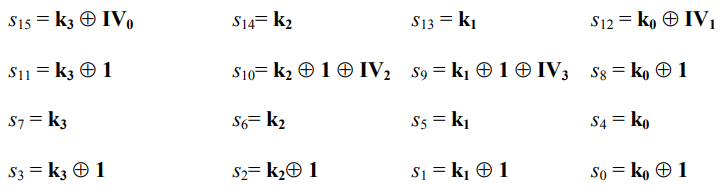
\includegraphics[width=0.75\linewidth]{Снимок экрана 2024-01-12 144510.png}
    \caption{Инициализация регистра [27]}
    \label{fig:enter-label}
\end{figure}

FSM инициализируется нулями: $R_1 = R_2 = R_3 = 0$. Затем производится следующие шаги в цикле 32 раз, не производя ключевой последовательности:

\begin{enumerate}
    \item FSM тактируется и выдает F.
    \item LSFR тактируется и добавляет в обновляемый бит F: $s_{t+16} = s_{t+16} \oplus F$ (при этом обычное вычисление обратной функции уже произошло).
\end{enumerate}

\textbf{Генерация ключевой последовательности}.

Пусть уже прошел этап инициализации. Сначала 1 раз тактируется FSM (его выход F никак не используется). Затем 1 раз тактируется LSFR (его выход никак не используется). Далее производится заданное количество $n$ 32-битных слов, повторяя следующие шаги $n$ раз: 

\begin{enumerate}
    \item FSM тактируется и выдает F.
    \item Выходное 32-битное слово вычисиляется как: $z_t = F \oplus s_0$.
    \item LSFR тактируется.
\end{enumerate}

\subsubsection{Безопасность шифра} 

Группа 3GPP провели многосторонний анализ безопасности Snow3G [28], пробуя применить разные атаки, особенно которые были эффективны против прошлых версии шифра. В результате они заключили, что шифр обеспечивает адекватную защиту конфиденциальности.

\section{SEAL}

Одним из важнейших параметров любого шифра является его скорость шифрования. Многие добивались этой скорости за счет аппаратно-ориентированных шифров и их аппаратной реализации. Phillip Rogaway и Don Coppersmith были следующей точки зрения: не всегда есть возможность купить криптографическое оборудование и использовать аппаратно-ориентированный шифр. Программная реализация таких шифров обычно существенно проигрывала в скорости и являлась непрактичной. Поэтому в 1993 году Rogaway и Don Coppersmith разработали потоковый шифр SEAL (Software-optimized Encryption Algorithm) [20], оптимизированный для программной реализации.

\subsubsection{Описание шифра SEAL}

SEAL является семейством псевдослучайных функций. Его параметрами являются: $a$ - 160-битный ключ, $n$ - 32-битная переменная (в алгоритме ее роль обычно играет счетчик сообщений) и $L$ - длина выходной последовательности. $SEAL(a, n, L)$ - семейством псевдослучайных функций, а $SEAL(a, *, L) = SEAL_{a, L}()$ - функция от параметра $n$, которая неотличима от случайной. Также авторы отмечают, что $a$ - может быть ключом переменной длины, просто стоит от него будет взять хэш-функцию $SHA-1$, чтобы спроецировать его в 160-битный ключ для SEAL. Предлагаемая схема шифрования потока сообщений $(m_1, m_2, \dots, m_N)$ такова: $c_i = (n, x \oplus SEAL(a, n, L))$, где $n$ - номер сообщения, а $L=|x|$.

Алгоритму на вход подаются: $(a, n, L)$. Сначала из $a$ - генерируются таблицы $T, R, S$ c помощью $SHA-1$ (подробннее об этом в [20]). Перед описанием основного алгоритма нужно ознакомиться с процедурой initialize:

\begin{figure}[H]
    \centering
    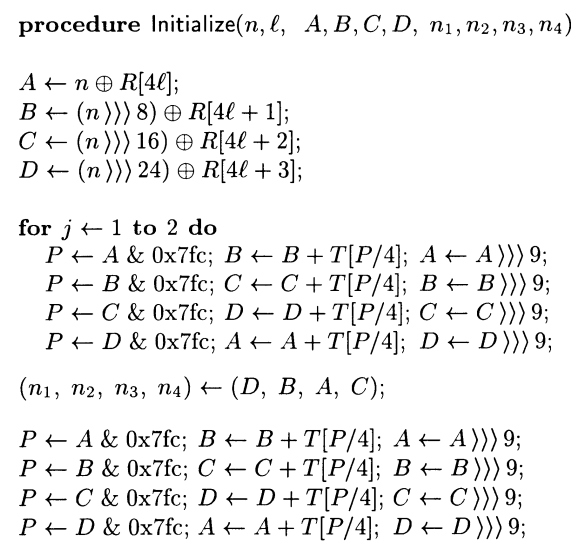
\includegraphics[width=0.5\linewidth]{init.png}
    \caption{Процедура initialize [20]}
    \label{fig:enter-label}
\end{figure}

Ей на вход подаются $n$ и $L$. По окончании процедуры устанвливаются значения для $A$, $B$, $C$, $D$, $n_1$, $n_2$, $n_3$ и $n_4$. Заметим, что перед этим таблицы $T$ и $R$ уже созданы с помощью $a$.

Основной алгоритм шифра SEAL:

\begin{figure}[H]
    \centering
    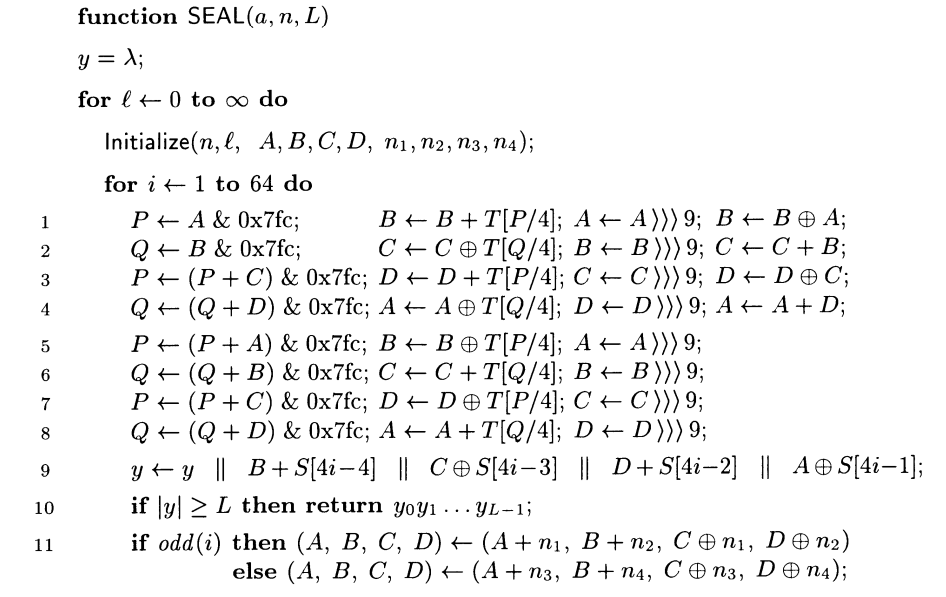
\includegraphics[width=0.75\linewidth]{Снимок экрана 2024-01-12 010838.png}
    \caption{Алгоритм шифра SEAL [20]}
    \label{fig:enter-label}
\end{figure}

Инициализация происходит каждые $32*4*64$ битов, пробегая по $l$. Параметр $L$ по факту является критерием останова. В строках 1-8 происходит генерация нашей псевдослучайной функции с помощью специальных констант, битовых операции, сложения 2 беззнаковых чисел и обращения к ранее вычисленным таблицам $T$ и $S$. Заметим, что для фиксированного $a$ и $n$, максимальное значение $L = 64 * 1024 * 8$ или 64 килобайта.

\subsubsection{Безопасность шифра} 

Авторы работы [21] смогли показать, что с помощью $2^{34}$ битов ключевой последовательности можно отличить SEAL от истинно случаной функцией. То есть SEAL не является псевдослучайной функцией. Позже начали появляться более надежные версии шифра SEAL.


\section{MUGI}

В 2002 году был создан генератор псевдослучаных чисел MUGI [22], в основе которого лежат принципы шифра PANAMA [23]. При разработке MUGI преследовалось 2 цели: 

\begin{enumerate}
    \item Шифр должен иметь возможность эффективно реализовываться на разном аппаратном оборудовании. 
    \item Сложность вычисления шифра должна быть меньше, чем у PANAMA.
\end{enumerate}

\subsubsection{Описание шифра MUGI}

MUGI получается на вход 2 параметра: 128-битный секретный ключ и 128-битный инициализирующий вектор. Каждый раунд шифр производит 64-битную ключевую последовательность. Входные параметры формируют состояние \textbf{a} и буфер \textbf{b}. Во время раунда $t$ состояние \textbf{a} и буфер \textbf{b} выглядят следующим образом: 

\begin{equation}
    \left\{\begin{array}{l}
\mathbf{a}^{(t)}=\left(a_0^{(t)}, a_1^{(t)}, a_2^{(t)}\right)\left(a_i^{(t)} \in \mathrm{GF}(2)^{64}\right) \\
\mathbf{b}^{(t)}=\left(b_0^{(t)}, \cdots, b_{15}^{(t)}\right)\left(b_i^{(t)} \in \mathrm{GF}(2)^{64}\right)
\end{array}\right.
\end{equation}

Инициализация \textbf{a(0)} и \textbf{b(0)} происходит с помощью секретного ключа и инициализирующего вектор (описание этого этапа находится в [22]). Выходом генератора в момент $t$ является: $Out[t] = a_2^(t)$, то есть второй юнит (вторые 64-бита) состояния \textbf{a(t)}.

\begin{figure}[H]
    \centering
    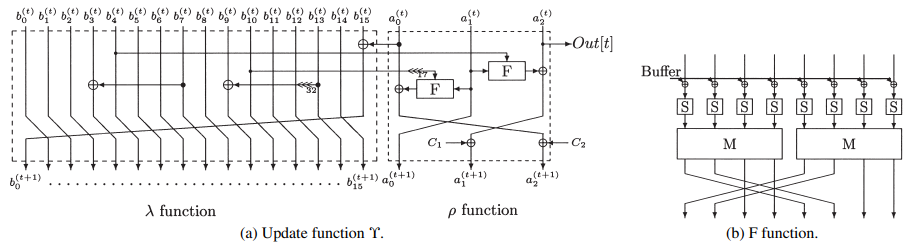
\includegraphics[width=1\linewidth]{Снимок экрана 2024-01-12 115522.png}
    \caption{Схема функций шифра MUGI [24]}
    \label{fig:enter-label}
\end{figure}

Каждый раунд происходит обновление \textbf{a} и \textbf{b} c помощью функции $\Upsilon$, $\lambda$, $\rho$ (они представлены на схеме выше) следующим образом:

\begin{equation}
    \left(\mathbf{a}^{(t+1)}, \mathbf{b}^{(t+1)}\right) =\Upsilon\left(\mathbf{a}^{(t)}, \mathbf{b}^{(t)}\right) 
=\left(\lambda\left(\mathbf{a}^{(t)}, \mathbf{b}^{(t)}\right), \rho\left(\left(\mathbf{a}^{(t)}, \mathbf{b}^{(t)}\right)\right)\right.
\end{equation}

\textbf{$\lambda$ function}.

\begin{equation}
    \begin{aligned}
& b_j^{(t+1)}=b_{j-1}^{(t)} \\
& b_0^{(t+1)}=b_{15}^{(t)} \oplus a_0^{(t)} \\
& b_4^{(t+1)}=b_3^{(t)} \oplus b_7^{(t)} \\
& b_{10}^{(t+1)}=b_9^{(t)} \oplus\left(b_{13}^{(t)} \lll 32\right)
\end{aligned}
\end{equation}

\textbf{$\lambda$ function}.

\begin{equation}
    \begin{aligned}
a_0^{(t+1)}= & a_1^{(t)} \\
a_1^{(t+1)}= & a_2^{(t)} \oplus \mathrm{F}\left(a_1^{(t)}, b_4^{(t)}\right) \oplus C_1 \\
a_2^{(t+1)}= & a_2^{(t)} \oplus \mathrm{F}\left(a_1^{(t)}, b_{10}^{(t)} \lll 17\right) \oplus C 2 \\
& C_1=0 x \mathrm{BB} 67 \mathrm{AE} 8584 \mathrm{CAA73B} \\
& C_2=0 x 3 \mathrm{C} 6 \mathrm{EF} 372 \mathrm{FE} 94 \mathrm{~F} 82 \mathrm{~B}
\end{aligned}
\end{equation}

S-box $S$ и матрица $M$ взяты из шифра AES.

\subsubsection{Безопасность шифра} 

Специалисты отмечают [25], что у буфера, который обновляется линейно, низкая линейная сложность - 32 и низкий период последовательнсоти - 48. Это создает риски восстановления секретного ключа. Также были найдены возможные уязвимости нелинейной компоненты - состояния \textbf{a} [26].

\section{Семейство шифров A5}

Семейство поточных шифров A5: A5/1, A5/2 и A5/3 используется в шифрования данных между телефоном и базовой станцией в европейской системе мобильной цифровой связи GSM (Groupe Spécial Mobile).

\subsection{A5/1} 

A5/1 представляет собой вторую по надежности версию алгоритма шифрования A5, применяемого в стандарте GSM для обеспечения конфиденциальности более чем 130 миллионов клиентов. Изначально шифр держался в секрете. Краткое описание дизайна A5/1 утекло в 1994 году, и устройство шифра было с получено с помощью обратной инженерии в 1999 году Брисеньо [3] на основе реального GSM-телефона.

A5/1 - потоковый шифр, основанный на трех линейных регистрах сдвига обратной связи, которые нерегулярно тактируются. Размер ключа составляет 64 бита, и последовательность ключей формируется путем выполнения операции XOR с выходами трех регистров.

\subsubsection{Устройство шифра A5/1}

Устройство A5/1 достаточно просто, его можно увидеть на следующей схеме:

\begin{figure}[H]
    \centering
    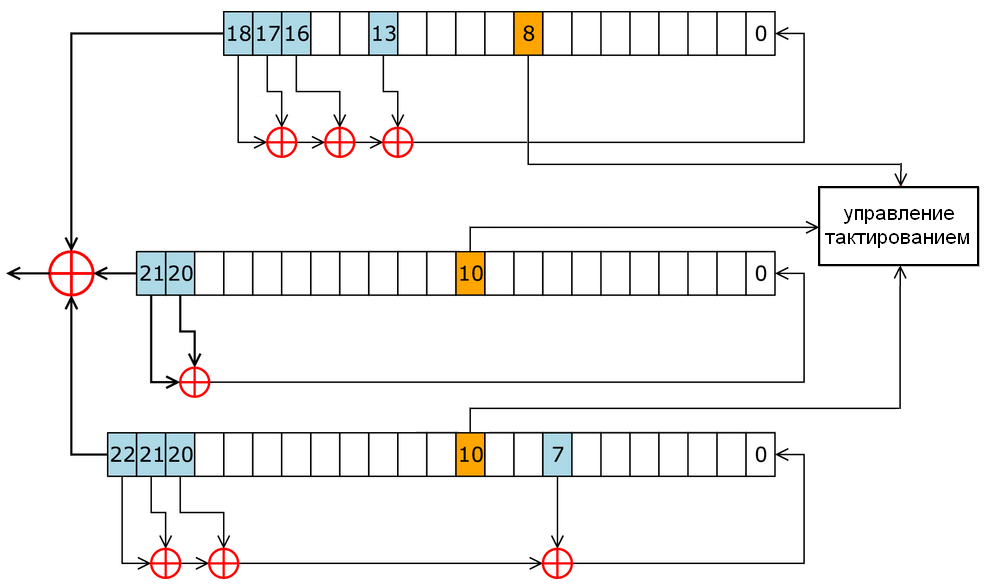
\includegraphics[width=0.5\linewidth]{РСЛОС_в_A5.png}
    \caption{Система регистров в алгоритме А5/1 [11]}
    \label{fig:enter-label}
\end{figure}

У нас есть три $LSFR$ $R_1$, $R_2$, $R_3$ длиной 19, 22, и 23 бита соотвественно. Они имеют следующие функции обратной связи:

$R_1$ : $x^{19} + x^{18} + x^{17} + x^{14} + 1$

$R_2$ : $x^{22} + x^{21} + 1$

$R_3$ : $x^{23} + x^{22} + x^{21} + x^{8} + 1$

Пусть регистры проинициализированы. Опишем 1 такт работы шифра:

\begin{enumerate}
        \item Берутся 3 бита из каждого регистра, 8-ой бит из $R_1$, 10-ой бит из $R_2$, 10-ой бит из $R_3$/.
        \item От этих 3 битов вычисляется функция $F=xy|xz|yz$.
        \item Тактирутся только те регистры, для которых полученное значение функции равно биту регистра, который подавался в фуннкцию F.
        \item Затем выходные биты региcтров cкладываются по модулю 2 и результат подается на выход генератора.
\end{enumerate}

\subsubsection{Функционирование шифра А5/1}.

Есть 64-битный регистр 

Данные в сеансе GSM передаются в виде последовательности кадров, где один кадр отправляется каждые 4,6 миллисекунды. Каждый кадр содержит 114 битов, идущих от A к B, и еще 114 битов, идущих от B к A. Каждый сеанс шифруется новым сеансовым ключом. Затем идет инициализация генератора, описание которой будет ниже. Затем генерируется 228 бит ключевой последовательности, которая накладывается на 228 битов открытого текста.

\textbf{Инициализация А5/1}.

На вход алгоритма подаются сеансовый 64-битный ключ K и 22-битный номер кадра $F_n$

\begin{enumerate}
        \item Обнуление регистров.
        \item 64 такта с регулярным тактированием, при которых очередной бит ключа складывается по модулю 2 с младшим битом каждого регистра и регистры сдвигаются
        \item аналогичные 22 такта, только с номером $F_n$
        \item 100 тактов с нерегулярным тактированием
\end{enumerate}

После инициализации генерируется ключевая последовательность длиной в 228 бит.

\subsubsection{Безопасность шифра} 

Одной из первых атак была атака компромисса между временем/памятью/данными [12] c вычислительной сложностью около $2^{40}-2^{45}$. В 2000 году была презентована новая атака компромисса между временем/памятью/данными [13], которая выполняется на персональном компьютере не дольше нескольких минут. Однако она требует 150-300 гигабайт памяти для своей таблицы. 

\subsection{A5/2}

A5/2 - синхронный потоковый шифр, который является модификацией шифра А5/1. А5/2 был специально разработан как экспортный вариант для стран, не входивших в Евросоюз. При этом криптостойкость модификации шифра является более низкой.

\subsubsection{Устройство шифра A5/2}

Устройство A5/2 имеет некоторые отличия от устройства А5/1:

\begin{figure}[H]
    \centering
    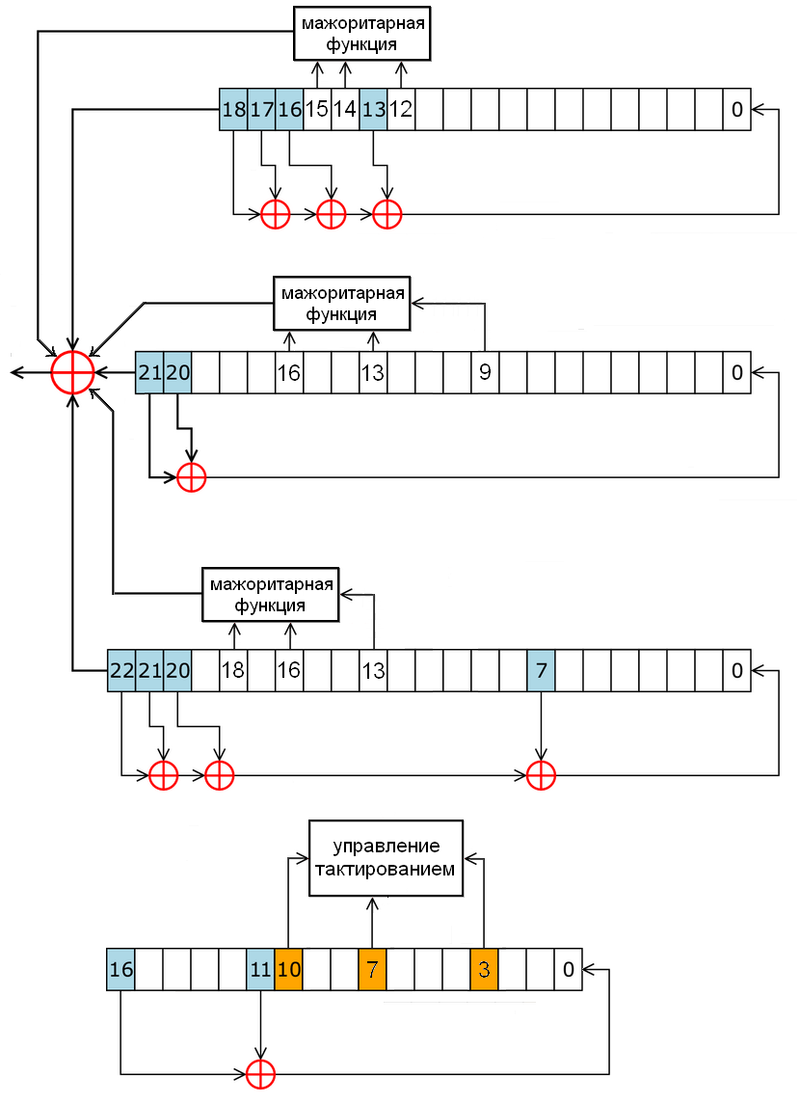
\includegraphics[width=0.5\linewidth]{РСЛОСвA52.png}
    \caption{Устройство А5/2 [14]}
    \label{fig:enter-label}
\end{figure}

У нас есть 4 $LSFR$ $R_1$, $R_2$, $R_3$, $R_4$ длиной 19, 22, 23, 17 бита соотвественно. Они имеют следующие функции обратной связи:

$R_1$ : $x^{19} + x^{18} + x^{17} + x^{14} + 1$

$R_2$ : $x^{22} + x^{21} + 1$

$R_3$ : $x^{23} + x^{22} + x^{21} + x^{8} + 1$

$R_4$ : $x^{17} + x^{12} + 1$

Пусть регистры проинициализированы. Опишем 1 такт работы шифра:

\begin{enumerate}
        \item Берутся 3 бита из регистра $R_4$: 3, 7 и 10.
        \item От этих 3 битов вычисляется функция голосования $F=xy|xz|yz$.
        \item $R_1$ тактируется, если 10-ый бит $R_4 = F$, $R_2$ тактируется, если 3-ий бит $R_4 = F$, $R_3$ тактируется, если 7-ой бит $R_4 = F$.
        \item Затем от каждого из первых трех регистров берется функция голосования для своих 3 битов: $R_1 - x_{12}, x_{14} \oplus 1, x_{15}$, $R_2 - x_{9}, x_{13}, x_{16} \oplus 1$, $R_3 - x_{13} \oplus 1, x_{16}, x_{18}$. Результаты этих функции суммируются по модулю 2 с выходными битами первых трех регистров. Полученное значение подается на выход генератора.
\end{enumerate}

\subsubsection{Функционирование шифра А5/2}

Такое же как и в А5/1.

\textbf{Инициализация А5/2}.

Инициализация претерпела изменения. На вход алгоритма подаются сеансовый 64-битный ключ K и 22-битный номер кадра $F_n$

\begin{enumerate}
        \item Обнуление регистров.
        \item 64 такта с регулярным тактированием, при которых очередной бит ключа складывается по модулю 2 с младшим битом каждого регистра ($R_1$, $R_2$, $R_3$ и $R_4$) и регистры сдвигаются.
        \item аналогичные 22 такта, только с номером $F_n$
        \item 1 такт 3 бита $R_4$ (3, 7, 10) заполняются единицами.
        \item 99 тактов с нерегулярным тактированием.
\end{enumerate}

После инициализации генерируется ключевая последовательность длиной в 228 бит.

\subsubsection{Безопасность шифра} 

Этот шифр не является безопасным. Например, есть атака, которая без дополнительных вычислений за секунды может взломать шифр [15].

\subsection{A5/3}

Около 20 лет алгоритмы А5/1 и А5/2 стояли на страже "безопасности" телефонных разговоров, эти шифры были недостаточно стойкими. Поэтому на смему им приходит новый блочный шифр KASUMI, который ложится в основу А5/3. KASUMI берет свои истоки из криптосистемы MISTY. 

После внедрения, A5/3 станет одной из наиболее широко используемых криптосистем в мире, и обеспечение её безопасности станет одним из наиболее важных практических вопросов в области криптографии.

\subsubsection{Описание KASUMI}

Этот алгоритм был опубликован в спецификации [16] в 2003 году. KASUMI - это сеть Фейстеля с 8 раундами. Он работает с блоком данных размером 64 бита и использует ключ размером 128 бит. Опишем функцию раунда $f_i$.

\textbf{Функция раунда $f_i$}. 

Функция раунда $f_i$ принимает 32-битный блок $I$, ключ раунда $RK_i = (KL_i, KO_i, KI_i)$. Функция $f_i$ зависит от раунда. Внутрии ее используются функции $FO$, $FL$ В 1,3,5,7 раундах она равна:
\begin{equation}
    f_i(I, RK_i) = FO(FL(I, KL_i), KO_i, KI_i)
\end{equation}

В 2,4,6,8 раундах она равна:
\begin{equation}
    f_i(I, RK_i) = FL(FO(I, KO_i, KI_i), KL_i)
\end{equation}

\textbf{Функция $FL$}.

Функция $FL$ принимает 32-битный блок $I=(L||R)$ и 32-битный подключ $KL_i = (KL_{i,1}||KL_{i,2})$.

\begin{enumerate}
    \item $R' = R \oplus ROL(L and KL_{i,1})$
    \item $L' = L \oplus ROL(R' or KL_{i,1})$
\end{enumerate}

$ROL$ это циклический сдвиг влево. Выходом функции является $(L'||R')$.

\textbf{Функция $FO$}.

Функция $FO$ принимает 32-битный блок $I=(L_0||R_0)$, 48-битный подключ $KO_i = KO_{i,1}||KO_{i,2}||KO_{i,3}$ и 48-битный подключ $KI_i = KI_{i,1}||KI_{i,2}||KI_{i,3}$.

Для $j=1,2,3$:

\begin{enumerate}
    \item $R_j = FI(L_{j-1} \oplus KO_{i,j}, KI_{i, j}) \oplus R_{j-1}$, функция $FI$, которая будет описана ниже
    \item $L_j = R_{j-1}$
\end{enumerate}

Выходом функции является $(L_3||R_3)$.

\textbf{Функция $FI$}.

Функция $FI$ принимает 16-битный блок $I=(L_0||R_0)$ и 16-битный подключ $KI_{i, j} = (KI_{i, j, 1}||KI_{i, j, 2})$. $L_0$ - 9 битов, $L_0$ - 7 битов. $KI_{i, j, 1}$ - 7 битов, $KI_{i, j, 2}$ - 9 битов. 

Также в функции $FI$ используются две подстановки: 7-битная $S7$ и 9-битная $S9$, которые представлены в [16]; две фукнции $ZE(x)$ и $TR(x)$: $ZE(x)$ -> $00||x$, $TR(x)$ -> $x[2:]$, то есть первая фукнция добавляет 2 нуля на место самых значимых битов, а вторая отрезает 2 самых значимых бита.  

\begin{enumerate}
    \item $L_1 = R_0$
    \item $R_1 = S9[L_0] \oplus ZE(R_0)$
    \item $L_2 = R_1 \oplus KI_{i, j, 2}$
    \item $R_2 = S7[L_1] \oplus TR(R_1) \oplus KI_{i, j, 1}$
    \item $L_3 = R_2$
    \item $R_3 = S9[L_2] \oplus ZE(R_2)$
    \item $L_4 = S7[L_3] \oplus TR(R_3)$
    \item $R_4 = R_3$
\end{enumerate}

Выходом функции является $(L_4||R_4)$.

\textbf{Расписание ключей}.

KASUMI имеет 128-битный ключ $K$. Каждый раунд используется 128-битный ключ, который высчитывается из $K$. Сначала считаются 2 16-битных массива $\{K_j\}$ и $\{K_{j'}\} (j=1 to 8)$ следующим образом. Первый массив это:

\begin{equation}
    K=K1||K2||K3||K4||K5||K6||K7||K8
\end{equation}

А второй массив равен изначально ключу плюс заданной маске ($K + mask$. Затем полученное значение также делится на 8 равных частей. Маску можно найти в [16]. И далее из этих массивов на каждом раунде считаются соотвествующие ключи: 

\begin{figure}[H]
    \centering
    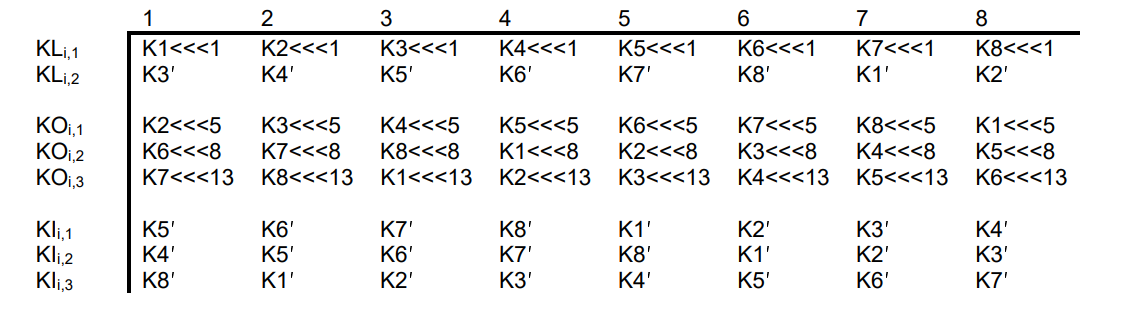
\includegraphics[width=0.75\linewidth]{Снимок экрана 2024-01-11 152806.png}
    \caption{Расписание ключей [16]}
    \label{fig:enter-label}
\end{figure}

\subsubsection{Функционирование алгоритма}

\textbf{Инициализация А5/1}. На вход подается 32-битный вектор CC, 5-битный вектор CB, 1-битный вектор CD, 8-битный вектор CA, 16-битный вектор CE. Эти вектора загружаются в 64-битный регистрc следующим образом: 

\begin{equation}
    A = CC||CB||CD||00||CA||CE
\end{equation}

Установим $KM = 0x55555555555555555555555555555555$, $KSB_0 = 0$. Далее 1 раз вызывается KASUMI для регистра А(блок) с подданным на иницилизацию секретным ключом СК:

\begin{equation}
    A = KASUMI[A]_{CK \oplus KM}
\end{equation}

Иницилизация завершена.

\textbf{Генерация ключевой последовательности}. Далее генируется N 64-битных блоков следующм образом, где BLKCNT - счетчик блоков, а СК - секретный ключ: 

\begin{equation}
    KSB_n = KASUMI[A \oplus BLKCNT \oplus KSB_{n-1}]_{CK}
\end{equation}

Количество блоков генерируется ровно столько, сколько надо для покрытия шифруемой последовательности (в GSM - 114 бит, в ECSD - 348 бит). Таким образом, мы получаем ключевую последовательность, составленную из блоков.

\subsubsection{Безопасность шифра}

В работе [18] 2010 года описывается сендвич-атака на KASUMI, которая проводится за $2^{32}$ операции. При этом они используют знания о 4 ключах и сообщениях, что делает атаку неприменимой к А5/3. Авторы отмечают, что целью их работы было показать, что переход от MISTY к KASUMI ослабил криптографическую стойкость шифра, так как MISTY на момент публикации не имел атак эффективнее, чем полный перебор ключа.

В одной из последних работ [19], выпущенной в 2022 году, авторы представили атаку на основе выбора открытых текстов, которая требует $2^{63}$ битов исходного текста, и $2^{63.3}$ операции шифрования, и некоторые условия на ключ. Вероятность успеха этой атаки $2^{-18}$. 

Таким образом, один из самых используемых потоковых шифров в мире имеет свои недостатки, однако для взлома требуется достаточно специфичные условия.

\section{Шифр LILI128}

\subsection{Описание} 

В 2000 году на NESSIE workshop был предложен шифр LILI128. LILI128 [1] это потоковый шифр, работающий в синхронном режиме и основанный на LSFR, с ключом в 128 бит. Разработчики утверждают, что у него большой период, большая линейная сложность, и что он устойчив к атакам, известным на 2002 год. 

Рассмотрим его устройство подробнее на следующей схеме:

\begin{figure}[H]
    \centering
    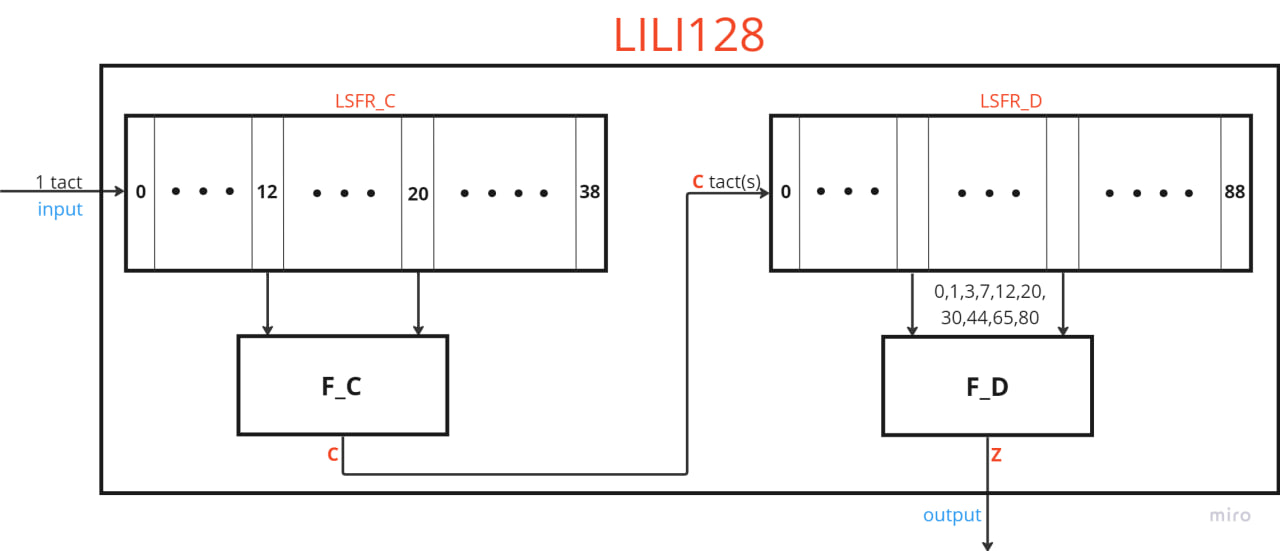
\includegraphics[width=0.8\linewidth]{my_lili_scheme.jpg}
    \caption{Устройство LILI128}
    \label{fig:enter-label}
\end{figure}

Шифр состоит из двух регистров $LSFR_C$ и $LSFR_D$, двух функции $f_c$ и $f_d$. Пусть регистры проинициализированы. Опишем 1 такт работы шифра:

\begin{enumerate}
        \item $LSFR_C$ производит 1 такт.
        \item У регистра $LSFR_C$ берутся значения в 13 и 21 ячейках и от них берется функция $f_c$. \newline $c = f_c(x_{12}, x_{20})$
        \item Регистр $LSFR_D$ производит $c$ тактов.
        \item У регистра $LSFR_D$ берутся значения в 1,2,4,8,13,21,31,45,66,81 ячейках и от них cчитается функция $f_d$. Выходом шифра на 1 такте является результат этой функции $f_d$.
\end{enumerate}

Функции шифра:
\begin{itemize}
    \item[$\blacksquare$]Функция $f_c(x_{12}, x_{20}) = 2*x_{12}+x_{20}+1$.
    \item[$\blacksquare$]Функция $f_d$ задана в виде таблицы, которая находится в приложении статьи [1].
    \item[$\blacksquare$]Функцией обратной связи для $LSFR_C$ является следующий примитивный полином:

    \begin{equation}
        x^{39}+x^{35}+x^{33}+x^{31}+x^{17}+x^{15}+x^{14}+x^2+1
    \end{equation}

    \item[$\blacksquare$]Функцией обратной связи для $LSFR_D$ является следующий примитивный полином:

    \begin{equation}
        x^{89}+x^{83}+x^{80}+x^{55}+x^{53}+x^{42}+x^{39}+x+1
    \end{equation}

\end{itemize}

Некоторые характеристики шифра:

\begin{itemize}
  \item[$\blacksquare$] Период выходной последовательности $z(t)$ равен $(2^{39}-1)(2^{89}-1) \approx 2^{128}$.
  \item[$\blacksquare$] Выходная последовательность $z(t)$ сбалансирована, то есть ее количество нулей  примерно равно ее количеству единиц (соотношение 1 к 0 равно $2^{88}$ : $2^{88}-1$).
  \item[$\blacksquare$] Линейная сложность выходной последовательность $z(t)$ не меньше, чем $2^{68}$
  \item[$\blacksquare$] Ненулевые ключи приводят к разным ключевым последовательностям. Хотя некоторые генераторы с нерегулярным тактированием при разных ключах выдают одну и ту же ключевую последовательность.
  \begin{remark}
    Нерегулярным тактированием регистра называется такое тактирование, при котором значение с регистра может сниматься как после 1 такта, так и после нескольких.
  \end{remark}
\end{itemize}

\subsection{Особенности реализации}

\textbf{Программная реализация}. Во время сдачи шифра на NESSIE workshop у авторов была реализация шифра LILI на языке С, которая работала со скоростью 4.8Мб/с (1200 циклов на байт) на 650МГц процессоре Pentium III с 128Мб ОЗУ. На момент написания статьи авторы добились скорости в 7.5Мб/с на той же машине. Первая реализация использовала конфигурацию Фиббоначи, а вторая - Галуа. При программной реализации конфигурация Галуа является более эффективной, так как состояние регистра складывается по модулю 2 с маской (которая содержит коэффициенты примитивного многочлена), а при Фиббоначи нужно складывать по модулю 2 все необходимые биты.

Авторы отмечают, что первоначальное вычисление маски Галуа приводит к дополнительным накладным расходам при инициализации, однако это происходит с незначительными затратами на скорость, так как это происходит только один раз.

Также приросту скорости второй реализации поспособствовал выбор размера слова процессора для виртуального регистра, типа unsigned (где это возможно), и побитового сдвига влево, вместо побитового сдвига вправо, так как он использовал меньше машинных инструкции.

\textbf{Возможности аппаратной реализации}. Для аппаратной реализации LSFR стоит использовать конфигурацию Фиббоначи. Для повышения скорости можно вместо нерегулярного тактирования поддерживать 4 копии функции обратной связи, с помощью которых можно перейти к регулярному тактированию. Авторы предпологают, что такая аппаратная реализация по производительности будет близка к скорости базового тактового генератора.



\subsection{Атаки}

В оригинальной статье [1] авторы утверждают, что для атаки "разделяй и властвуй" требуется минимум $2^{112}$ операции и 1700 битов ключевой последовательности. Также авторы утверждают, что на момент создания шифра не существовало быстрых корреляционных атак на нерегулярно тактируемый регистр. Меньше чем через год Fredrik Jönsson и Thomas Johansson опубликовали быструю корреляционную атаку [3], которая требовала операции меньше чем $2^{112}$.

\subsubsection{Быстрая корреляционная атака от Fredrik Jönsson и Thomas Johansson}

В своей статье [3] авторы демонстрируют быструю корреляционную атаку на LILI128, которая требует около $2^{71}$ битовых операции при условии, что известна ключевая последовательность длиной около $2^{30}$, и проведена фаза предварительных вычислений, количество которых равно $2^{79}$. Основная концепция атаки была взята из более общей работы [5].

\textbf{Угроза и модель нарушителя}. Данная атака направлена на получение k битов начального состояния регистра $LSFR_d$, где k - является параметром. После удачной атаки таким же образом происходит восстанавливание всего начального состояния $LSFR_d$. 

Это атака на основе знания открытого текста (known-plaintext attack, KPA), так как нарушитель знает ключевую последовательность, что эквивалентно знанию пар открытого текста и шифротекста.

\textbf{Описание атаки}.

\textbf{\emph{Постановка}}. Предположим, что у нас есть ключевая последовательность длины N $z = (z_1, z_2, \dots, z_N)$. Пусть выходная последовательность $f_d$ будет $d = (d_1, d_2, \dots, d_M)$, где $M > N$, когда $LSFR_d$ регулярно тактируется. Обозначим номера тактов $LSFR_d$ \space $s = (s_1, s_2, \dots, s_N)$, которые берутся как выходные биты.

\begin{equation}
    z_k = d_{s_k}, \space k = 1, \dots, N
\end{equation}

Предполагается значение регистра $LSFR_c$ и по нему высчитывается $s = (s_1, s_2, \dots, s_N)$. Если это значение верно то: $z = (d_{s_1}, d_{s_2}, \dots, d_{s_N}$. Далее по этой последовательности ищется начальное состояние регистра $LSFR_d$. Обозначим последовательность, произведенную $LSFR_d$ при регулярном тактировании, $u = (u_1, u_2, \dots, u_N)$. Из нее мы получаем $d_i$, следуя описанию шифра (Рисунок 3):

\begin{equation}
    d_i = f_d(u_{i-89}, u_{i-88}, u_{i-86}, u_{i-79}, u_{i-77}, u_{i-69}, u_{i-59}, u_{i-45}, u_{i-24}, u_{i-9})
\end{equation}

Далее требуется аппроксимировать $f_d$ линейной функцией.

\textbf{\emph{Аппроксимация $f_d$}}. Быстрые корреляционные атаки основаны на теории кодов, исправляющих ошибки [6]. Фильтрующая или комбинирущая функция, которая используется в шифрах, основанных на LSFR, интерпретируется как бинарный симметричный канал, через который передается информация. Функцию $f_d$ необходимо аппроксимировать линейной, для того чтобы составить уравнения проверки паритета (parity check equations) [6].

 Для этого необходимо произвести преобразование Уолша (Walsh Transform): 
\begin{equation}
        F(\omega)=\sum_x(-1)^{f(x) \oplus \omega \cdot x}
\end{equation}

Также через него выражается нелинейность булевой функции:
\begin{equation}
        N_f=2^{n-1}-\frac{1}{2} \max _\omega|F(\omega)|
\end{equation}

В статье [1] написано, что $N_{f_d} = 480$. Следовательно мы можем найти линейную функцию $f_l(x_1, x_2, \dots, x_{10} = a_1*x_1+a_2*x_2+ \dots +a_{10}*x_{10}$, такую что $d_H(f_d, f_l) = 480$. Если так аппроксимировать функцию, то мы получаем что: 

\begin{equation}
    p = P\left(f_d(x)=f_l(x)\right)=\frac{1024-480}{1024}=0.53125
\end{equation}

Разложив функцию $f_d$ на спектр Уолша, мы получаем, что существует 240 функции, таких что $d_H(f_d, f_l) = 480$. Для атаки берутся все функции.

\textbf{\emph{Предварительные вычисления}}. Далее идет модификация алгоритма [5] с параметром t=3. Множество L всех состоянии $LSRF_d$ длиной 89 имеет мощность $|L|=2^{89}$ и последовательность фиксированной длины N, полученная из состояния из L, является линейным-[N, 89] кодом C с матрицей генератором $G_{LSFR_d}$.

Заменив $f_d$ на одну из $f_l$, мы можем записать выход $f_l$ как линейную комбинацию начального состояния $u_0$. Таким образом, мы можем найти матрицу $G^{89*N}$, с помощью которой выходная последовательность $v$, полученную из $f_l$, записывается как $v = u_0 * G$.

Так как линейных функции 240 $f_{l_1}, f_{l_2}, \dots, f_{l_240}$, то мы можем построить 240 матриц генераторов
$G_1, G_2, \dots, G_{240}$, которая конкетинируется в большую матрицу $G'$ размером $89*240N$:

\begin{equation}
    G' = (G_1, G_2, \dots, G_240) = (g_1, g_2, \dots, g_{240N})
\end{equation}

Следуя алгортирму [5], выбирается параметр k < 89. Находятся все тройки стобцов $g_{i_1}, g_{i_2}, g_{i_3}$, таких что:

\begin{equation}
\left(\boldsymbol{g}_{i_1}+\boldsymbol{g}_{i_2}+\boldsymbol{g}_{i_3}\right)^{\mathrm{T}}=(\underbrace{*, *, \ldots, *}_k, \underbrace{0,0, \ldots, 0}_{89-k})
\end{equation}, где $*$ означает любое значение (но не все нули).

\textbf{\emph{Поиск первых k битов регистра $LSFR_d$ по ключевой последовательности}}. Пусть таких троек будет $m$. Для каждой такой тройки считается $v_{i_1} + v_{i_2} + v_{i_3}$, которая является линейной комбинацией только первых k символов изначального состояния и не зависит от остальных 89 - k других символов. Таким образом, формируется новый линейный-[m, k] код: 

\begin{equation}
    (v_{i_1(1)} + v_{i_2(1)} + v_{i_3(1)}, v_{i_1(2)} + v_{i_2(2)} + v_{i_3(2)}, \dots, v_{i_1(3)} + v_{i_2(3)} + v_{i_3(3)})
\end{equation}

По этим же тройкам из ключевой последовательности формируется новая, равная зашумленной последовательности, сгенерированной из последнего линейного-[m, k] кода:

\begin{equation}
    Z = (Z_1, Z_2, \dots, Z_m), Z_j = (z_{i_1(j)} + z_{i_2(j)} + z_{i_3(j)}), 1 <= j <= m
\end{equation}

Здесь же можно посчитать вероятность ошибки $e$ переданного кода. $z_i = v_i + e_i$, где $e_i$ случайная двоичная величина c: 

\begin{equation}
    P(e_i = 1) = p = P(z_i \neq v_i) = 1 - 0.53125 => \epsilon = 0.03125.
\end{equation}

А для переданного кода (полученного из троек): 

\begin{equation}
    p_3 = P(e_{i_1(j)} + e_{i_2(j)} + e_{i_3(j)} = 1) = 3p(1-p)+p^3 = 1/2 - 4*\epsilon^2 \approx 0.49988
\end{equation}

Это означает, что зашумленная последовательность почти не коррелирует с изначальной. Это усложняет сложность но атаки, но оставляет ее возможной.

Последним шагом из последного полученного кода полным перебором среди векторов длины k находится кодовое слово ближайшее к $Z = (Z_1, Z_2, \dots, Z_m)$. Заметим что кодовое слово получается из вектора длины k, умноженного на матрицу генератор. Таким образом, первые k битов ближайшого кодового слова являются искомыми битами начального состояния при должной длине ключевой последовательности. Остальные биты начального состояния ищутся также, например, можно искать следующие k битов. Последующий поиск будет намного быстрее, так как на самом деле в первой итерации мы также перебираем полное начальное состояне $LSFR_c$ и в следующей итерации этого делать не надо. 

Описаный выше алгоритм описан для регулярно тактируемого $LSFR_d$, который в LILI128 нерегулярно тактируется. Поэтому сведем задачу к предыдущей. Перед выдачей бита с регистра $LSFR_d$ тактируется в среднем 2.5 раза, поэтому $M \approx 2.5N$. Поэтому в фазе предварительных вычислений мы рассматриваем все $240M$ возможнных символов при конструкции линейного-[m, k] кода, из которых затем выбираем $240N$ символов c помощью последовательности $s$, получившейся из $LSFR_c$ из фиксированного состяния. И наконец, этот алгоритм выполняется для каждого возможного состояния $LSFR_c$. Поэтому мы и получаем после первой итерации $39 + k$ битов общего начального состояния шифра LILI128.

\textbf{\emph{Оценка требуемых ресурсов для атаки}}. Приведем основные результаты расчетов из [3]. Для t = 3 желательная длина N равна: 

\begin{equation}
    N \approx \frac{1}{960} \cdot(k \cdot 12 \cdot \ln 2)^{1 / 3} \cdot \varepsilon^{-2} \cdot 2^{(89-k) / 3}
\end{equation}

Количество требуемых операции при этом равно:

\begin{equation}
    2^k*k*\frac{2*ln2}{(2\epsilon)^{2t}}
\end{equation}

Для шифра LILI128 c $l=89$, $\epsilon=0.03125$ и $t=3$ была получена следующая таблица, в котором для некоторых $k$ расчитаны $N$ и количество требуемых операции для декодирования $C_{dec}$:

\begin{figure}[H]
    \centering
    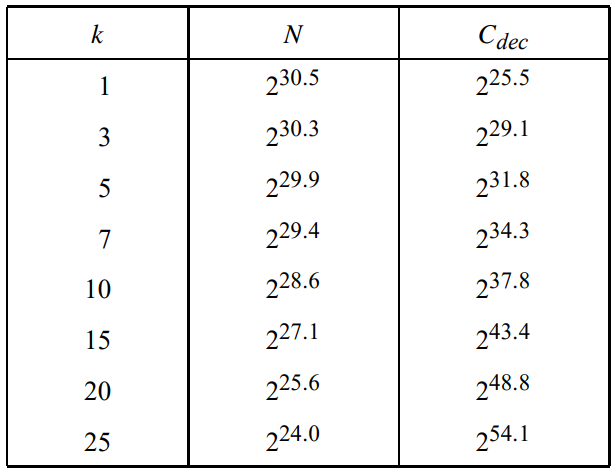
\includegraphics[width=0.5\linewidth]{Снимок экрана 2024-01-09 112308.png}
    \caption{Желательная длина ключевой последовательности $N$ и количество требуемых операции для декодирования $C_{dec}$ для заданного $k$ и начального состояния $LSFR_c$} [3]
    \label{fig:enter-label}
\end{figure}

Для k=5 нужно около $2^{32}$ операции. Учитывая перебор по начальным состяниям $LSFR_c$ получается то, что суммарная вычислительная сложность атаки равна $2^{39}*2^{32} = 2^{71}$. При этом необходима ключевая последоватльность размера 128Мб. Фаза предварительных вычислений требует $2^{79}$ операции.

\textbf{\emph{Возможности практической реализации атаки}}. В 2023 году на cамом мощном суперкомпьютере с частотой в 1600 петафлопс атака проводится за 24 минуты. Очевидно, что в 2002 году это атака еще не представляла угрозы. На тот момент она имела важный теоритический результат, так как авторы шифра LILI128 были не правы, оценив сложность корреляционной атаки минимум в $2^{112}$ операции.

\textbf{\emph{Пути нейтрализации атаки}}. В данной атаке, одним из основных параметров, определяющих сложность является $\epsilon$. Поэтому если мы выберем фильтрующую функцию с нелинейностью больше, чем 480, то мы существенно увеличим сложность атаки.


\subsubsection{Time-memory tradeoff atack на LILI128}

Через 8 месяцев после публикации [3] Saarinen M. J. O. публикуют новую атаку [8], которая также опровергает утверждения разработчиков LILI128 о его безопасности. Это атака компромисса между временем/памятью/данными, которая обходит один защитных методов шифра - нерегулярное тактирование.

\textbf{Угроза и модель нарушителя}. Данная атака направлена на получение всего начального состояния регистра $LSFR_d$.

Это атака на основе знания открытого текста (known-plaintext attack, KPA), так как нарушитель знает ключевую последовательность, что эквивалентно знанию пар открытого текста и шифротекста.

Ознакомимся с леммами из статьи [8] без доказательства:

\begin{lemma}
    При совершении $\Delta_c = 2^{39}-1$ тактов $LFSR_c$, происходит ровно $\Delta_d = 5*2^{38} - 1$ тактов $LFSR_d$.
\end{lemma}

\begin{lemma}
    Существует матрица размера $89 * 89$, такая что при умножении на нее вектора начального состояния $LSFR_d$ мы получим состояние $LSFR_d$, тактированное на $\Delta_d$ шагов от изначального. Аналогично есть матрица, которая отматывает регистр назад на $\Delta_d$ шагов от текущего. Для расчета такой матрицы потребутся около $2^{38}$ битовых операции.
\end{lemma}

\textbf{Описание атаки}.

\textbf{\emph{Предварительный этап}}. Строится таблица, содержащая $2^{45}$ пар вида (89-битное слово, 45-битное слово). Каждая пара считается следующим образом. Берется случайный вектор длиной 89 и загружается в $LSFR_d$, из него семплируются 45 битов, которые в выходной последовательности находятся на расстоянии  $\Delta_d$. Семплирование происходит с помощью умножения начального состояния на специальную матрицу (см. Лемма 4.1)

Индексом таблицы является 45-битное слово, которое может быть получено из разных начальных состоянии, поэтому могут быть коллизии. Ожидаемая заполненность таблицы равна $1 - \exp{-2}=0.8647$. Ее размер - $2^{51.48}$. Вычислительная сложность построения - $2^{48}$ операции алгоритма Data Encryption Standard (DES).

\textbf{\emph{Фаза просмотра таблицы}}. Пусть у нас есть $2^{46}$ битов ключевой последовательности $z(0), z(1), \dots, z(2^{46}-1)$

\begin{figure}[H]
    \centering
    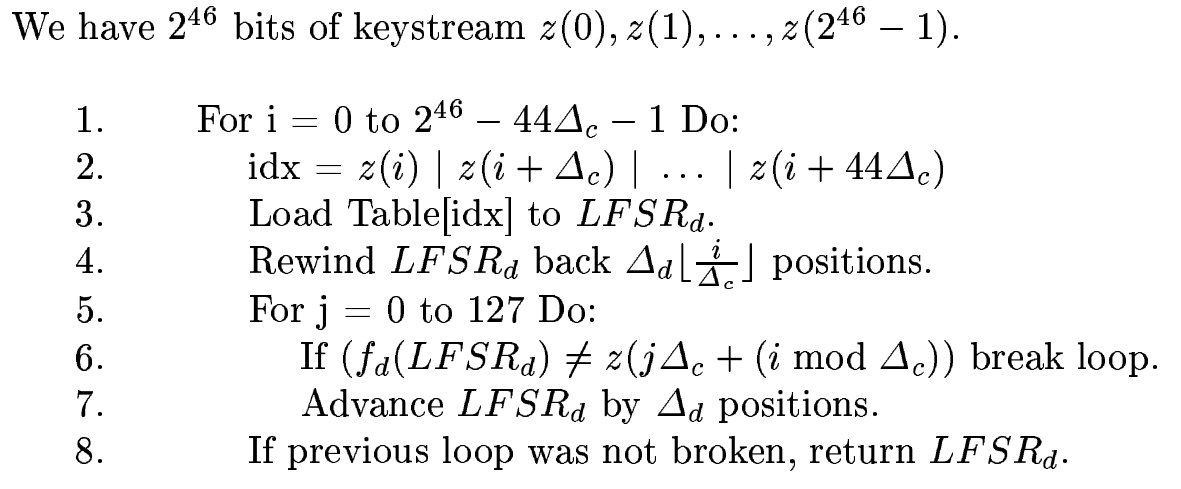
\includegraphics[width=0.5\linewidth]{Снимок.PNG}
    \caption{Алгоритм атаки [8]}
    \label{fig:enter-label}
\end{figure}

В первой строчке мы пробегаемся по всем подпоследовательностям $z$ длины 45, элементы которых находятся на расстоянии $\Delta_c$ друг от друга. В 2ой строчке берем очередную подпоследовательность. Далее ищем ее в нашей таблице, при успехе вытаскиваем соотвествующее начальное значение регистра $LSFR_d$, иначе следущая итерация. Затем откатываем состояние регистра на число кратное $\Delta_d$, если i перескочило через $\Delta_c$. В строчках 5-7 мы проверяем совпадает ли сгенерированная из $LSFR_d$ 128-битная последовательность (с шагом в $\Delta_d$) с наблюдаемой $z$ (с шагом $\Delta_c$). И если она совпала, то возвращаем текущее начальное состояние регистра.

Вероятность того, что состояние будет верным равно:

\begin{equation}
    1-\left(1-\frac{0.8647 * 2^{45}}{2^{89}}\right)^{2^{46}-44 \Delta_c} \approx 90 \%
\end{equation}

\textbf{\emph{Оценка требуемых ресурсов для атаки}}. Для атаки требуется $2^{46}$ битов ключевой последовательности. Таблица размером размером - $2^{51.48}$ бит, вычислительная сложность ее построения - $2^{48}$ операции алгоритма DES.

\textbf{\emph{Возможности практической реализации атаки}}. Вычислительная сложность в $2^{48}$ операции алгоритма DES более чем позволяет ее провести при условии, что есть необходимый объем ключевой последовательности. Но проблема в том, что собрать $2^{46}$ битов ключевой последовательности в большинстве случаев невозможно. Поэтому если эта атака и применима, то только в таких специфичных случаях, когда доступен "неограниченный" объем ключевой последовательности.

\textbf{\emph{Пути нейтрализации атаки}}. С помощью увеличения длины атакуемого регистра можно существенно затруднить данную атаку, так как вырастет объем таблицы и количество требуемых опереаций.

\subsubsection{Атака на фильтрующую функцию}
В 2007 году китайские исследователи [9] смогли получить явный вид функции $f_d$ шифра LILI128. Для этого им понадобилось около $2^{12}-2^{13}$ битов ключевой последовательности. Реконструкция функции была проведена на IBM ноутбуке с помощью MATLAB за 1.6 часов.

\textbf{Угроза и модель нарушителя}. Данная атака направлена на фильтрующую функцию $f_d$ шифра LILI128. Злоумышленник проводит реконструкцию функции $f_d$, что упрощает дальнейший криптоанализ.

Нарушитель имеет доступ к оракулу шифрования. Он сам его инициализирует, использует и далее анализирует полученную ключевую последовательность. Также он знает, что выход шифра - это выход какой-то фильтрующей функции $f_d$. То есть в их атаке неизвестной переменной является только функция $f_d$, хотя обычно целью атаки является начальное состояние. Поэтому модель нарушителя не совсем вписывается в общепринятые модели.

\textbf{Описание атаки}. Авторы не приводят точного алгоритма атаки, но описывают основные приемы, которые были применены.
    Первым шагом они взяли программную имплементацию шифра и проинициализировали ее значением "yyyyyyyyyyyyyyyy". Затем сгенерировали ключевую последователность. И взяли из нее такой отрезок последовательности (начиная с первого бита), который бы выражал функцию $f_d$ и был бы минимален по сложности (вероятно имеется в виду линейная сложность). Это они могли сделать с помощью знания того, от каких конкретно позиции состояния $LSFR_d$ берется функция $f_d$. Затем с помощью кластеризации и нелинейного прогноза они смогли восстановить диаграмму фазового пространства, состоящей из 10 измерений: (1, 2, 3, 4, 5, 6, 7, 8, 9, 10), из ключевой последовательности, полученной на предыдущем шаге. Реконструированная в АНФ $f_d$ содержит 46 слагаемых, как линейные так и нелинейные:

    \begin{equation}
        \begin{aligned}
    x_2 & +x_3+x_4+x_5+x_6 x_7+x_1 x_8+x_2 x_8+x_1 x_9+x_3 x_9 \\
    & +x_4 x_{10}+x_6 x_{10}+x_3 x_7 x_9+x_4 x_7 x_9+x_6 x_7 x_9+x_3 x_8 x_9 \\
    & +x_6 x_8 x_9+x_4 x_7 x_{10}+x_5 x_7 x_{10}+x_6 x_7 x_{10}+x_3 x_8 x_{10} \\
    & +x_4 x_8 x_{10}+x_2 x_9 x_{10}+x_3 x_9 x_{10}+x_4 x_9 x_{10}+x_5 x_9 x_{10} \\
    & +x_3 x_7 x_8 x_{10}+x_5 x_7 x_8 x_{10}+x_2 x_7 x_9 x_{10}+x_4 x_7 x_9 x_{10} \\
    & +x_6 x_7 x_9 x_{10}+x_1 x_8 x_9 x_{10}+x_3 x_8 x_9 x_{10}+x_4 x_8 x_9 x_{10} \\
    & +x_6 x_8 x_9 x_{10}+x_4 x_6 x_7 x_9+x_5 x_6 x_7 x_9+x_2 x_7 x_8 x_9 \\
    & +x_4 x_7 x_8 x_9+x_4 x_6 x_7 x_9 x_{10}+x_5 x_6 x_7 x_9 x_{10} \\
    & +x_3 x_7 x_8 x_9 x_{10}+x_4 x_7 x_8 x_9 x_{10}+x_4 x_6 x_7 x_8 x_9 \\
    & +x_5 x_6 x_7 x_8 x_9+x_4 x_6 x_7 x_8 x_9 x_{10}+x_5 x_6 x_7 x_8 x_9 x_{10}
    \end{aligned}
    \end{equation}

    Непосредственной проверкой можно проверить, что полученная функция и функция $f_d$, заданная таблицей в оригинальной статье совпадают.

    Также авторы утверждают, что если видоизменить функцию $f_d$, задать начальное 128-битное состояние, сгенерировать ключевую последовательность длиной $2^{13}$ и отравить им, то они смогут ее реконструировать.

    Это атака не дает возможности узнать начальное состяние. Но явный вид функции открывает новые вектора атаки на функцию с меньшей вычислительной сложностью, что позже и сделали. В 2012 году была придумана атака [10], которая существенно эффективнее, чем предыдущие. Она требует $2^{47}$ предварительных вычислений, которые создают таблицу размером $2^{47}$ 89-битных слов, ключевую последовательность длиной $2^{46}$ битов  и $2^{35}$ активных вычислений. 

    \textbf{\emph{Оценка требуемых ресурсов для атаки}}. Для атаки требуется $2^{13}$ битов ключевой последовательности. Количество требуемых операции не приведено, но реконструкция функции была проведена на IBM ноутбуке с помощью MATLAB за 1.6 часов.
    
    \textbf{\emph{Возможности практической реализации атаки}}. Атака реализована.
    
    \textbf{\emph{Пути нейтрализации атаки}}. Так как нету точного алгоритма атаки, то труднее понять, как от нее защититься. Авторы ищут явный функции, поэтому можно предположить, что если увеличить количество переменных, от которых зависит функция, то мы существенно увеличим количество требуемых операции для реконструкции.

\subsection{Заключение}

Шифр LILI128 имеет достаточно простую конструкцию, его можно эффективно реализовать как программно, так и аппаратно. Он имеет большой период, сбалансированную выходную ключевую последовательность и высокую линейную сложность. Но авторы явно ошиблись в оценке защищенности шифра, так как почти сразу после публикации шифра вышла быстрая корреляционная атака, которая имела сложность ниже, чем нижняя оценка сложности авторов. Также специалисты в ряде атак (например [8]) смогли обойти нерегуляруемое тактирование, которое тоже было добавлено как элемент усиливающий безопаность шифра. Наконец, китайские исследователи [9] смогли получить явный вид функции $f_d$, что открыло новые векторы атак и существенно понизило безопаность шифра. Учитывая количество уязвимостей генератора LILI128, тяжело назвать его безопасным. Он не является CPA-стойким, однако объем ключевой последовательности, которую необходимо собрать для атаки является достаточно большим.

\section{Список литературы}

[1] Clark A. et al. The LILI-II keystream generator // Information Security and Privacy: 7th Australasian Conference, ACISP 2002 Melbourne, Australia, July 3–5, 2002 Proceedings 7. – Springer Berlin Heidelberg, 2002. – С. 25-39.

[2] Dubrova E. How to speed-up your NLFSR-based stream cipher //2009 Design, Automation and Test in Europe Conference and Exhibition. – IEEE, 2009. – С. 878-881.

[3] Jönsson F., Johansson T. A fast correlation attack on LILI-128 //Information Processing Letters. – 2002. – Т. 81. – №. 3. – С. 127-132

[4] Siegenthaler. Decrypting a class of stream ciphers using ciphertext only //IEEE Transactions on computers. – 1985. – Т. 100. – №. 1. – С. 81-85.

[5] Chepyzhov V. V., Johansson T., Smeets B. A simple algorithm for fast correlation attacks on stream ciphers //Fast Software Encryption: 7th International Workshop, FSE 2000 New York, NY, USA, April 10–12, 2000 Proceedings 7. – Springer Berlin Heidelberg, 2001. – С. 181-195.

[6] MacWilliams F. J., Sloane N. J. A. The theory of error-correcting codes. – Elsevier, 1977. – Т. 16.

[7] Babbage S. H. Improved" exhaustive search" attacks on stream ciphers //European Convention on Security and Detection, 1995. – IET, 1995. – С. 161-166.

[8] Saarinen M. J. O. A time-memory tradeoff attack against LILI-128 //Fast Software Encryption: 9th International Workshop, FSE 2002 Leuven, Belgium, February 4–6, 2002 Revised Papers 9. – Springer Berlin Heidelberg, 2002. – С. 231-236.

[9] Huang X. et al. Reconstructing the nonlinear filter function of LILI-128 stream cipher based on complexity //arXiv preprint cs/0702128. – 2007.

[10] Mihaljević M. J. et al. Internal state recovery of keystream generator LILI-128 based on a novel weakness of the employed Boolean function //Information Processing Letters. – 2012. – Т. 112. – №. 21. – С. 805-810.

[11] Баданин М.Ф. . - URL: https://commons.wikimedia.org/wiki/File:РСЛОС\_в\_A5.png (дата обращения: 28.12.2023)

[12] Golić J. D. Cryptanalysis of alleged A5 stream cipher //International Conference on the Theory and Applications of Cryptographic Techniques. – Berlin, Heidelberg : Springer Berlin Heidelberg, 1997. – С. 239-255.

[13] Biryukov A., Shamir A., Wagner D. Real time cryptanalysis of A5/1 on a PC //Fast Software Encryption: 7th International Workshop, FSE 2000 New York, NY, USA, April 10–12, 2000 Proceedings 7. – Springer Berlin Heidelberg, 2001. – С. 1-18.

[14] Баданин М.Ф. . - URL: https://commons.wikimedia.org/wiki/File:РСЛОСвA52.png (дата обращения: 28.12.2023) 

[15] Bogdanov A., Eisenbarth T., Rupp A. A hardware-assisted realtime attack on A5/2 without precomputations //Cryptographic Hardware and Embedded Systems-CHES 2007: 9th International Workshop, Vienna, Austria, September 10-13, 2007. Proceedings 9. – Springer Berlin Heidelberg, 2007. – С. 394-412.

[16] 3rd Generation Partnership Project, Technical Specification Group Services and
System Aspects, 3G Security, Specification of the 3GPP Confidentiality and Integrity Algorithms; Document 2: KASUMI Specification, V3.1.1, 2001.

[17] Amirki . - URL: https://commons.wikimedia.org/wiki/File:Feistel\_cipher\_diagram\_en.svg (дата обращения: 29.12.2023) 

[18] Dunkelman O., Keller N., Shamir A. A practical-time attack on the A5/3 cryptosystem used in third generation GSM telephony //Cryptology ePrint Archive. – 2010.

[19] Sugio N., Igarashi Y., Hongo S. Integral Cryptanalysis on Reduced-Round KASUMI //IEICE Transactions on Fundamentals of Electronics, Communications and Computer Sciences. – 2022. – Т. 105. – №. 9. – С. 1309-1316.

[20] Rogaway P., Coppersmith D. A software-optimized encryption algorithm //Fast Software Encryption: Cambridge Security Workshop Cambridge, UK, December 9–11, 1993 Proceedings 1. – Springer Berlin Heidelberg, 1994. – С. 56-63.

[21] Handschuh H., Gilbert H. χ2 cryptanalysis of the SEAL encryption algorithm //International Workshop on Fast Software Encryption. – Berlin, Heidelberg : Springer Berlin Heidelberg, 1997. – С. 1-12.

[22] Watanabe D. et al. A new keystream generator MUGI //Fast Software Encryption: 9th International Workshop, FSE 2002 Leuven, Belgium, February 4–6, 2002 Revised Papers 9. – Springer Berlin Heidelberg, 2002. – С. 179-194.

[23] Daemen J., Clapp C. Fast hashing and stream encryption with PANAMA //International Workshop on Fast Software Encryption. – Berlin, Heidelberg : Springer Berlin Heidelberg, 1998. – С. 60-74.

[24] Sekine H. et al. A strength evaluation of a pseudorandom number generator MUGI against linear cryptanalysis //IEICE transactions on fundamentals of electronics, communications and computer sciences. – 2005. – Т. 88. – №. 1. – С. 16-24.

[25] Golić J. D. A weakness of the linear part of stream cipher MUGI //Fast Software Encryption: 11th International Workshop, FSE 2004, Delhi, India, February 5-7, 2004. Revised Papers 11. – Springer Berlin Heidelberg, 2004. – С. 178-192.

[26] Biryukov A., Shamir A. Analysis of the non-linear part of MUGI //Fast Software Encryption: 12th International Workshop, FSE 2005, Paris, France, February 21-23, 2005, Revised Selected Papers 12. – Springer Berlin Heidelberg, 2005. – С. 320-329.

[27] ETSI/SAGE. Specification of the 3GPP Confidentiality and Integrity Algorithms UEA2 and UIA2. Document 2: SNOW 3G Specification, version 1.1 (September 2006)

[28] ETSI/SAGE. Specification of the 3GPP Confidentiality and
Integrity Algorithms UEA2 & UIA2.
Document 5: Design and Evaluation Report, version 1.1 (September 2006)

[29] Klein A. Attacks on the RC4 stream cipher //Designs, codes and cryptography. – 2008. – Т. 48. – С. 269-286.

[30] Paul G., Rathi S., Maitra S. On non-negligible bias of the first output byte of RC4 towards the first three bytes of the secret key //Designs, Codes and Cryptography. – 2008. – Т. 49. – С. 123-134.

[31] Vanhoef M., Piessens F. All Your Biases Belong to Us: Breaking {RC4} in {WPA-TKIP} and {TLS} //24th USENIX Security Symposium (USENIX Security 15). – 2015. – С. 97-112.

 \end{document}
